%
% Grizzards Complete Guide
%
% If you're a human, skip to "\mainmatter" to skip over the preamble.
%
\documentclass[10pt,twocolumn]{memoir}

\setstocksize{11in}{8.5in}
\settrimmedsize{\stockheight}{\dimexpr 8.5in-15mm}{*}

\setlrmarginsandblock{.333333in}{.5in}{*}
\setulmarginsandblock{.75in}{.75in}{*}
\setheadfoot{.5in}{.5in}
\widowpenalty=10000
\clubpenalty=10000

\makeevenfoot{plain}{\thepage}{}{}
\makeoddfoot{plain}{}{}{\thepage}

\usepackage[utf8]{inputenc}
\usepackage{babel}
\usepackage{stfloats}
\usepackage{microtype}
\usepackage{graphicx}
\usepackage{pdfpages}
\tolerance=1
\emergencystretch=\maxdimen
%\usepackage{tgtermes}
\usepackage{hyperref}
\usepackage{xcolor}
\hypersetup{
    colorlinks,
    linkcolor={black},
    citecolor={blue!50!black},
    urlcolor={blue!80!black},
    pdftitle={Grizzards Complete Guide},
    pdfsubject={Grizzards videogame for the Atari 2600},
    pdfauthor={Bruce-Robert Pocock}%,
%    pdfkeywords={Your PDF keywords}
  }
\usepackage{caption}
\captionsetup{labelformat=empty}

\usepackage{tikz}

\newcommand\encircle[1]{%
  \tikz[baseline=(X.base)] 
  \node (X) [draw, shape=circle, inner sep=.25pt] {#1};}

\newcommand\pic[1]{%
  \begin{center}
    \includegraphics[interpolate,width=.333\columnwidth]{../Manual/#1.png}
  \end{center}}

\newcommand\bigpic[1]{%
  \begin{center}
    \includegraphics[interpolate,width=\columnwidth]{../Manual/#1.png}
  \end{center}}

\setlength{\columnsep}{.333333in}
%% \setlength\columnseprule{.5pt}

\usepackage{lettrine}
%\usepackage[protrusion=true,expansion=true]{microtype}
\fontfamily{pnc}
\chapterstyle{komalike}

\checkandfixthelayout

\title{Grizzards Complete Guide}
\author{Bruce-Robert Pocock}

\newcommand{\listmapname}{List of Maps}
\newlistof{listofmaps}{map}{\listmapname}

%
%
%
%%% BEGIN DOCUMENT
%
%
%

\begin{document}

\frontmatter

\maketitle

\thispagestyle{empty}

\chapter*{Introduction}\label{Introduction}

The  land of  Syrex  is  a dangerous  place.  Fierce  monsters roam  the
countryside. But luckily for you, you're a Grizzard handler!

\bigskip

This guide  contains a  complete guide  to the  \textit{Grizzards} game,
including spoilers.

\vspace{1in}\vfill

This is the \textit{Grizzards} Complete Guide.

\vspace{12pt}

The  \textit{Grizzards} videogame  software,  including its  audiovisual
components and this guide, are copyright \copyright{} 2022, Bruce-Robert
Pocock. All Rights are Reserved except as granted under license.

\bigskip

This videogame software was not created, published, or licensed by Atari
or its successors.

\vspace{12pt}

Published by AtariAge. \href{https://atariage.com/}{https://atariage.com/}

\bigskip

You are hereby granted permission  to make use of the \textit{Grizzards}
videogame software for \emph{non-commercial personal use}.

Redistribution not for profit is allowed, but sales of this software
requires a license.

\let\cleardoublepage\clearpage

\mainmatter

\setcounter{secnumdepth}{3}
\tableofcontents

\newenvironment{grizzardpage}[6]{{%

    \vfill
  \section{#1}\label{grizzard:#1}

  Grizzard number: #2

  \subsection*{Starting Stats}

  \begin{description}
  \item[Attack]
    #4
  \item[Defend]
    #5
  \item[Maximum Hit Points]
    #3
  \end{description}

  \subsection*{Moves}

  See page~\pageref{sec:GrizzardMoves} for a guide to all the Grizzards' moves.

  \subsection*{Metamorphosis}

  \ifx\relax\detokenize{#6}\relax {

    #1 does not metamorphose (it is a final form).

  }\else {

    #1 will metamorphose into  #6 (see page~\pageref{grizzard:#6}) after
    gaining 27 experience points.

  }\fi

  \subsection*{Description}

}{}}

\chapter{Grizzards}

There  are 30  different  Grizzards  that you  can  catch  and train  in
the  game.  Each   Grizzard  has  its  own  statistics   and  can  learn
different Moves. 

\begin{grizzardpage}{Dirtex}{01}{10}{1}{1}{Lander}

  Dirtex  is one  of the  Starter  Grizzards that  you can  choose at  the
  beginning of the game. A green anole-like Grizzard, it is native to dry,
  desert regions. Dirtex's Moves tend to be more aggressive than the other
  two Starters.

\end{grizzardpage}

\begin{grizzardpage}{Aquax}{02}{10}{1}{1}{Sailor}

  Aquax  is one  of  the Starter  Grizzards  that you  can  choose at  the
  beginning of the game. A brown  alligator-like Grizzard, it is native to
  swamps.  Of the  three Starters,  Aquax  is the  most balanced  Grizzard
  between attacking and defending Moves.

\end{grizzardpage}

\begin{grizzardpage}{Airex}{03}{10}{1}{1}{Flyer}

Airex  is one  of  the Starter  Grizazrds  that you  can  choose at  the
beginning  of  the  game.  A  teal  gecko-like  Grizzard,  it  lives  in
the treetops. Airex's Moves are  more focused on buffing, debuffing, and
healing Moves than the other two Starters.
  
\end{grizzardpage}

\begin{grizzardpage}{Flamex}{04}{20}{6}{4}{Burner}

Flamex can be found in the Fire Bog.
  
\end{grizzardpage}

\begin{grizzardpage}{Petty}{05}{30}{1}{1}{Tyrant}

  Petty is found near  the foot of the cliffs on the  south side of Port
  Lion, to the west of the paths that lead up the cliffs.

  While  Petty  is  a  surprisingly  weak Grizzard  at  first,  it  does
  metamorphose into  one of the stronger  Grizzards — Tyrant —  and from
  there,  eventually  can become  the  very  strongest Grizzard  of  all
  — Megax. Training Petty is a  difficult exercise, but it pays off well
  in the end.

\end{grizzardpage}

\begin{grizzardpage}{Wetnas}{06}{15}{6}{4}{}

Wetnas is  found on the narrow  road leading from Treble  Village to the
south, just  north of the Lost  Mine's entrance. For most  players, this
will   be   the  first   Grizzard   that   you'll  catch,   after   your
Starter Grizzard.

While Wetnas's  stats are an improvement  over the Starters, and  it has
better Moves,  there are  advantages to returning  to Treble  Village to
switch  back to  your Starter  Grizzard —  in particular,  they tend  to
metamorphose  into  better Grizzards  than  Wetnas  if you  continue  to
train them.
  
\end{grizzardpage}

\begin{grizzardpage}{Windoo}{07}{20}{6}{4}{}
  WRITEME
\end{grizzardpage}

\begin{grizzardpage}{Firend}{08}{30}66{Dufont}
  WRITEME
\end{grizzardpage}

\begin{grizzardpage}{Lander}{09}{30}88{Zendex}
  WRITEME
\end{grizzardpage}

\begin{grizzardpage}{Sailor}{10}{30}88{Oceax}
  WRITEME
\end{grizzardpage}

\begin{grizzardpage}{Flyer}{11}{30}88{Flitex}
  WRITEME
\end{grizzardpage}

\begin{grizzardpage}{Burner}{12}{30}{10}{8}{Flarex}
  WRITEME
\end{grizzardpage}

\begin{grizzardpage}{Splodo}{13}{5}{75}{15}{}
  WRITEME
\end{grizzardpage}

\begin{grizzardpage}{Tyrant}{14}{60}{30}{40}{Megax}
  WRITEME
\end{grizzardpage}

\begin{grizzardpage}{Dufont}{15}{30}{15}{15}{Wapow}
  WRITEME
\end{grizzardpage}

\begin{grizzardpage}{Theref}{16}{50}{45}{55}{}
  WRITEME
\end{grizzardpage}

\begin{grizzardpage}{Cornet}{17}{30}{15}{15}{Uptrix}
  Cornet is  one of several  Grizzards found in  a cave north  of Anchor
  Village. You'll need a special key to unlock it.
\end{grizzardpage}

\begin{grizzardpage}{Ambren}{18}{40}{20}{20}{Altrix}
  Ambren is  one of several  Grizzards found in  a cave north  of Anchor
  Village. You'll need a special key to unlock it.
\end{grizzardpage}

\begin{grizzardpage}{Noctis}{19}{40}{20}{20}{Ectrix}
  Noctis is  one of several  Grizzards found in  a cave north  of Anchor
  Village. You'll need a special key to unlock it.
\end{grizzardpage}

\begin{grizzardpage}{Corlyn}{20}{40}{20}{20}{Ortrix}
  Corlyn can  be found hidden in  the eastern limits of  the Lion Woods.
  You may have to search for a while to reveal it.
\end{grizzardpage}

\begin{grizzardpage}{Wapow}{21}{45}{24}{24}{}
  WRITEME
\end{grizzardpage}

\begin{grizzardpage}{Zendex}{22}{45}{25}{25}{}
  WRITEME
\end{grizzardpage}

\begin{grizzardpage}{Oceax}{23}{45}{25}{25}{}
  WRITEME
\end{grizzardpage}

\begin{grizzardpage}{Flitex}{24}{45}{25}{25}{}
  WRITEME
\end{grizzardpage}

\begin{grizzardpage}{Flarex}{25}{50}{25}{25}{}
  WRITEME
\end{grizzardpage}

\begin{grizzardpage}{Uptrix}{26}{75}{37}{37}{}
  WRITEME
\end{grizzardpage}

\begin{grizzardpage}{Altrix}{27}{75}{37}{37}{}
  WRITEME
\end{grizzardpage}

\begin{grizzardpage}{Ectrix}{28}{75}{37}{37}{}
  WRITEME
\end{grizzardpage}

\begin{grizzardpage}{Ortrix}{29}{75}{37}{37}{}
  WRITEME
\end{grizzardpage}

\begin{grizzardpage}{Megax}{30}{90}{90}{90}{}
  Megax is the biggest, meanest Grizzard there is.
\end{grizzardpage}

\chapter{Monsters}\label{ch:Monsters}

The world of Syrex has been  invaded by hordes of monsters. Each monster
has its own Moves and statistics.

The statistics  for a monster  are raised when  you play in  Expert mode
(with the  Left Difficulty Switch  in the  ``A'' position), or  when you
encounter the  monster in New Game  Plus mode. In the  tables below, the
Enhanced value is  used in \emph{either} Expert mode  \emph{or} New Game
Plus. The  Severe value  is used  when playing  New Game  Plus \emph{in}
Expert Mode.



In addition,  nearly all monsters can  grow to Boss forms.  (Some unique
monsters \emph{only} occur in Boss forms, however.) Boss forms also have
enhanced statistics.

\newcommand\twice[1]{\the\numexpr#1*2\relax}
\newcommand\thrice[1]{\the\numexpr#1*3\relax}
\newcommand\fourx[1]{\the\numexpr#1*4\relax}
\newcommand\eightx[1]{\the\numexpr#1*8\relax}

\newenvironment{monsterpage}[5]{{
    \vspace{24pt}
    
    \section{#1}

    \subsection*{Base Stats}

    \begin{tabular}{l c c c}
      {} & Basic Mode & Enhanced & Severe \\
      Normal Attack & #2 & \twice{#2} & \fourx{#2} \\
      Normal Defend & #3 & \twice{#3} & \fourx{#3} \\
      Normal Hit Points & #4 & \twice{#4} & \fourx{#4} \\ \\
      Boss Attack & \twice{#2} & \fourx{#2} & \eightx{#2} \\
      Boss Defend & \twice{#3} & \fourx{#3} & \eightx{#3} \\
      Boss Hit Points & \twice{#4} & \fourx{#4} & \eightx{#4} \\
    \end{tabular}

    \subsection*{Points Earned}

    \begin{tabular}{l c c c}
      {} & Basic Mode & Enhanced & Severe \\
      Normal & #5 & \twice{#5} & \thrice{#5} \\
      Boss & \twice{#5} & \thrice{#5} & \fourx{#5}
    \end{tabular}
    
    \subsection*{Moves}

    See page~\pageref{sec:MonsterMoves} for a guide to all the monsters' moves.

    \subsection*{Description}
    
  }{}}

\newenvironment{bosspage}[5]{{
    \vspace{24pt}
    
    \section{#1}

    #1 only appears in Boss form.
    
    \subsection*{Base Stats}

    \begin{tabular}{l c c c}
      {} & Basic Mode & Enhanced & Severe \\
      Boss Attack & \twice{#2} & \fourx{#2} & \eightx{#2} \\
      Boss Defend & \twice{#3} & \fourx{#3} & \eightx{#3} \\
      Boss Hit Points & \twice{#4} & \fourx{#4} & \eightx{#4} \\
    \end{tabular}

    \subsection*{Points Earned}

    \begin{tabular}{l c c c}
      {} & Basic Mode & Enhanced & Severe \\
      Boss & \twice{#5} & \thrice{#5} & \fourx{#5}
    \end{tabular}
    
    \subsection*{Moves}

    See page~\pageref{sec:MonsterMoves} for a guide to all the monsters' moves.

    \subsection*{Description}
  }{}}

\begin{monsterpage}{Anubis Jackal}{58}{58}{60}{150}

%\pic{Anubis-Jackal}
  
  Guardians of  the underworld,  the Anubis  Jackals roam  the Labyrinth
  looking for lost souls.
  
\end{monsterpage}

\begin{monsterpage}{Bigger Crab}{47}{47}{50}{130}

%  \pic{Bigger-Crab}
  
  WRITEME
\end{monsterpage}

\begin{bosspage}{Boss Bear}{40}{40}{127}{2500}

%  \pic{Boss-Bear}
  
  WRITEME
\end{bosspage}

\begin{monsterpage}{Butter Fly}{36}{36}{39}{100}

  \pic{Butterfly}
  
  WRITEME
\end{monsterpage}

\begin{monsterpage}{Cave Bat}{18}{18}{20}{50}

  \pic{Cave-Bat}
  
  WRITEME
\end{monsterpage}

\begin{bosspage}{Cave Grue}{16}{16}{17}{50}
  \pic{Cave-Grue}
  
  WRITEME
\end{bosspage}

\begin{monsterpage}{Crazy Fox}{25}{26}{27}{70}
  \pic{Crazy-Fox}
  
  WRITEME
\end{monsterpage}

\begin{monsterpage}{Crazy Skull}{56}{56}{58}{150}
%  \pic{Crazy-Skull}
  
  WRITEME
\end{monsterpage}

\begin{monsterpage}{Creepy Spider}{28}{28}{29}{80}
  \pic{Creepy-Spider}
  
  WRITEME
\end{monsterpage}

\begin{monsterpage}{Devil Skull}{43}{42}{46}{120}
  WRITEME
\end{monsterpage}

\begin{bosspage}{Dragon Andrew}{25}{25}{75}{750}

  The weakest  of the  three dragons,  the Evil  Dragon Andrew  is still
  a difficult boss  to defeat. His lair's entrance is  in the north-west
  corner of the labyrinth.
  
\end{bosspage}

\begin{bosspage}{Dragon Fred}{30}{30}{87}{1000}

  The Dreaded  Dragon Fred  is more  difficult to  defeat than  the Evil
  Dragon  Andrew,  but  not  as   tough  as  the  Wicked  Dragon  Timmy.
  Fred's lair is found near the south-west corner of the labyrinth.

\end{bosspage}

\begin{bosspage}{Dragon Timmy}{35}{35}{100}{1250}

  The Wicked Dragon Timmy is the hardest of the three Dragons to defeat.
  His lair is found in the center of the Labyrinth.
  
\end{bosspage}

\begin{monsterpage}{Fierce Raptor}{38}{38}{40}{100}

  WRITEME
\end{monsterpage}

\begin{monsterpage}{Fire Drake}{42}{42}{44}{110}
  WRITEME
\end{monsterpage}

\begin{monsterpage}{Fire Panda}{10}{10}{12}{30}
  \pic{Fire-Panda}
  
  WRITEME
\end{monsterpage}

\begin{monsterpage}{Flame Doggo}{6}{7}{8}{30}
  \pic{Flame-Doggo}
  
  WRITEME
\end{monsterpage}

\begin{monsterpage}{Flying Skull}{50}{50}{52}{130}
  WRITEME
\end{monsterpage}

\begin{monsterpage}{Giant Bat}{52}{52}{55}{140}
  WRITEME
\end{monsterpage}

\begin{monsterpage}{Giant Crab}{32}{32}{35}{90}
  WRITEME
\end{monsterpage}

\begin{monsterpage}{Giant Slime}{48}{48}{51}{130}
  WRITEME
\end{monsterpage}

\begin{monsterpage}{Giant Spider}{57}{57}{59}{150}
  WRITEME
\end{monsterpage}

\begin{monsterpage}{Grabby Crabby}{34}{34}{36}{90}
  WRITEME
\end{monsterpage}

\begin{monsterpage}{Great Wyrm}{51}{51}{54}{150}
  WRITEME
\end{monsterpage}

\begin{monsterpage}{Horrid Slime}{2}{2}{4}{8}
  \pic{Horrid-Slime}
  
  WRITEME
\end{monsterpage}

\begin{monsterpage}{Lectro Sheep}{39}{39}{38}{110}
  WRITEME
\end{monsterpage}

\begin{monsterpage}{Leggy Mutant}{40}{40}{43}{110}
  \pic{Leggy-Mutant}
  
  WRITEME
\end{monsterpage}

\begin{monsterpage}{Man Bull}{46}{46}{48}{120}
  WRITEME
\end{monsterpage}

\begin{monsterpage}{Maze Jaguar}{54}{54}{56}{140}
  WRITEME
\end{monsterpage}

\begin{bosspage}{Mean Robber}{29}{29}{31}{80}
  WRITEME
\end{bosspage}

\begin{monsterpage}{Metal Mouse}{30}{30}{32}{80}
  \pic{Metal-Mouse}
  
  WRITEME
\end{monsterpage}

\begin{monsterpage}{Radish Goblin}{26}{26}{28}{70}
  \pic{Radish-Goblin}
  
  WRITEME
\end{monsterpage}

\begin{bosspage}{One-Eyed Cyclops}{22}{22}{24}{60}
  WRITEME
\end{bosspage}

\begin{monsterpage}{Poison Asp}{44}{44}{47}{120}
  WRITEME
\end{monsterpage}

\begin{monsterpage}{Rodent Of Unusual Size (R.O.U.S.)}{7}{8}{9}{35}
  \pic{R.O.U.S.}
  
  WRITEME
\end{monsterpage}

\begin{monsterpage}{Round Robin}{6}{6}{8}{20}
  \pic{Round-Robin}
  
  WRITEME
\end{monsterpage}

\begin{monsterpage}{Scary Rat}{43}{43}{44}{120}
  WRITEME
\end{monsterpage}

\begin{monsterpage}{Sky Mutant}{4}{5}{6}{20}
  \pic{Sky-Mutant}
  
  WRITEME
\end{monsterpage}

\begin{monsterpage}{Turnip Goblin}{44}{44}{45}{120}
  WRITEME
\end{monsterpage}

\begin{monsterpage}{Uber Slime}{55}{55}{57}{150}
  WRITEME
\end{monsterpage}

\begin{monsterpage}{Viking Turtle}{23}{24}{25}{70}
  WRITEME
\end{monsterpage}

\begin{monsterpage}{Venom Sheep}{20}{20}{21}{60}
  \pic{Venom-Sheep}
  
  WRITEME
\end{monsterpage}

\begin{monsterpage}{Vorpal Bunny}{12}{12}{15}{40}
  \pic{Vorpal-Bunny}
  
  WRITEME
\end{monsterpage}

\begin{monsterpage}{Water Kitty}{33}{33}{34}{90}
  \pic{Water-Kitty}
  
  WRITEME
\end{monsterpage}

\begin{monsterpage}{Wicked Slime}{2}{1}{2}{5}
  \pic{Wicked-Slime}
  
  WRITEME
\end{monsterpage}

\begin{monsterpage}{Will-O-Wisp}{14}{14}{2}{40}
  \pic{Will-O-Wisp}
  
  WRITEME
\end{monsterpage}

\chapter{Places}\label{ch:Places}

The world of Syrex can be considered to have three main areas:

\begin{itemize}
\item the Mainland,
\item the island of Port Lion,
\item and the Underworld.
\end{itemize}

Each area has its own distinct musical theme.

You  might also  notice that  when you're  above-ground, the  map screen
shows a  lighter colored ground  (compared to  the walls), but  when you
travel underground, the walls are lighter than the ground. 

\listofmaps

\clearpage
\thispagestyle{empty}
\begin{tikzpicture}[overlay, remember picture]
  \node[anchor=north west, xshift=-4pt, yshift=4pt] 
  at (current page.north west)
  {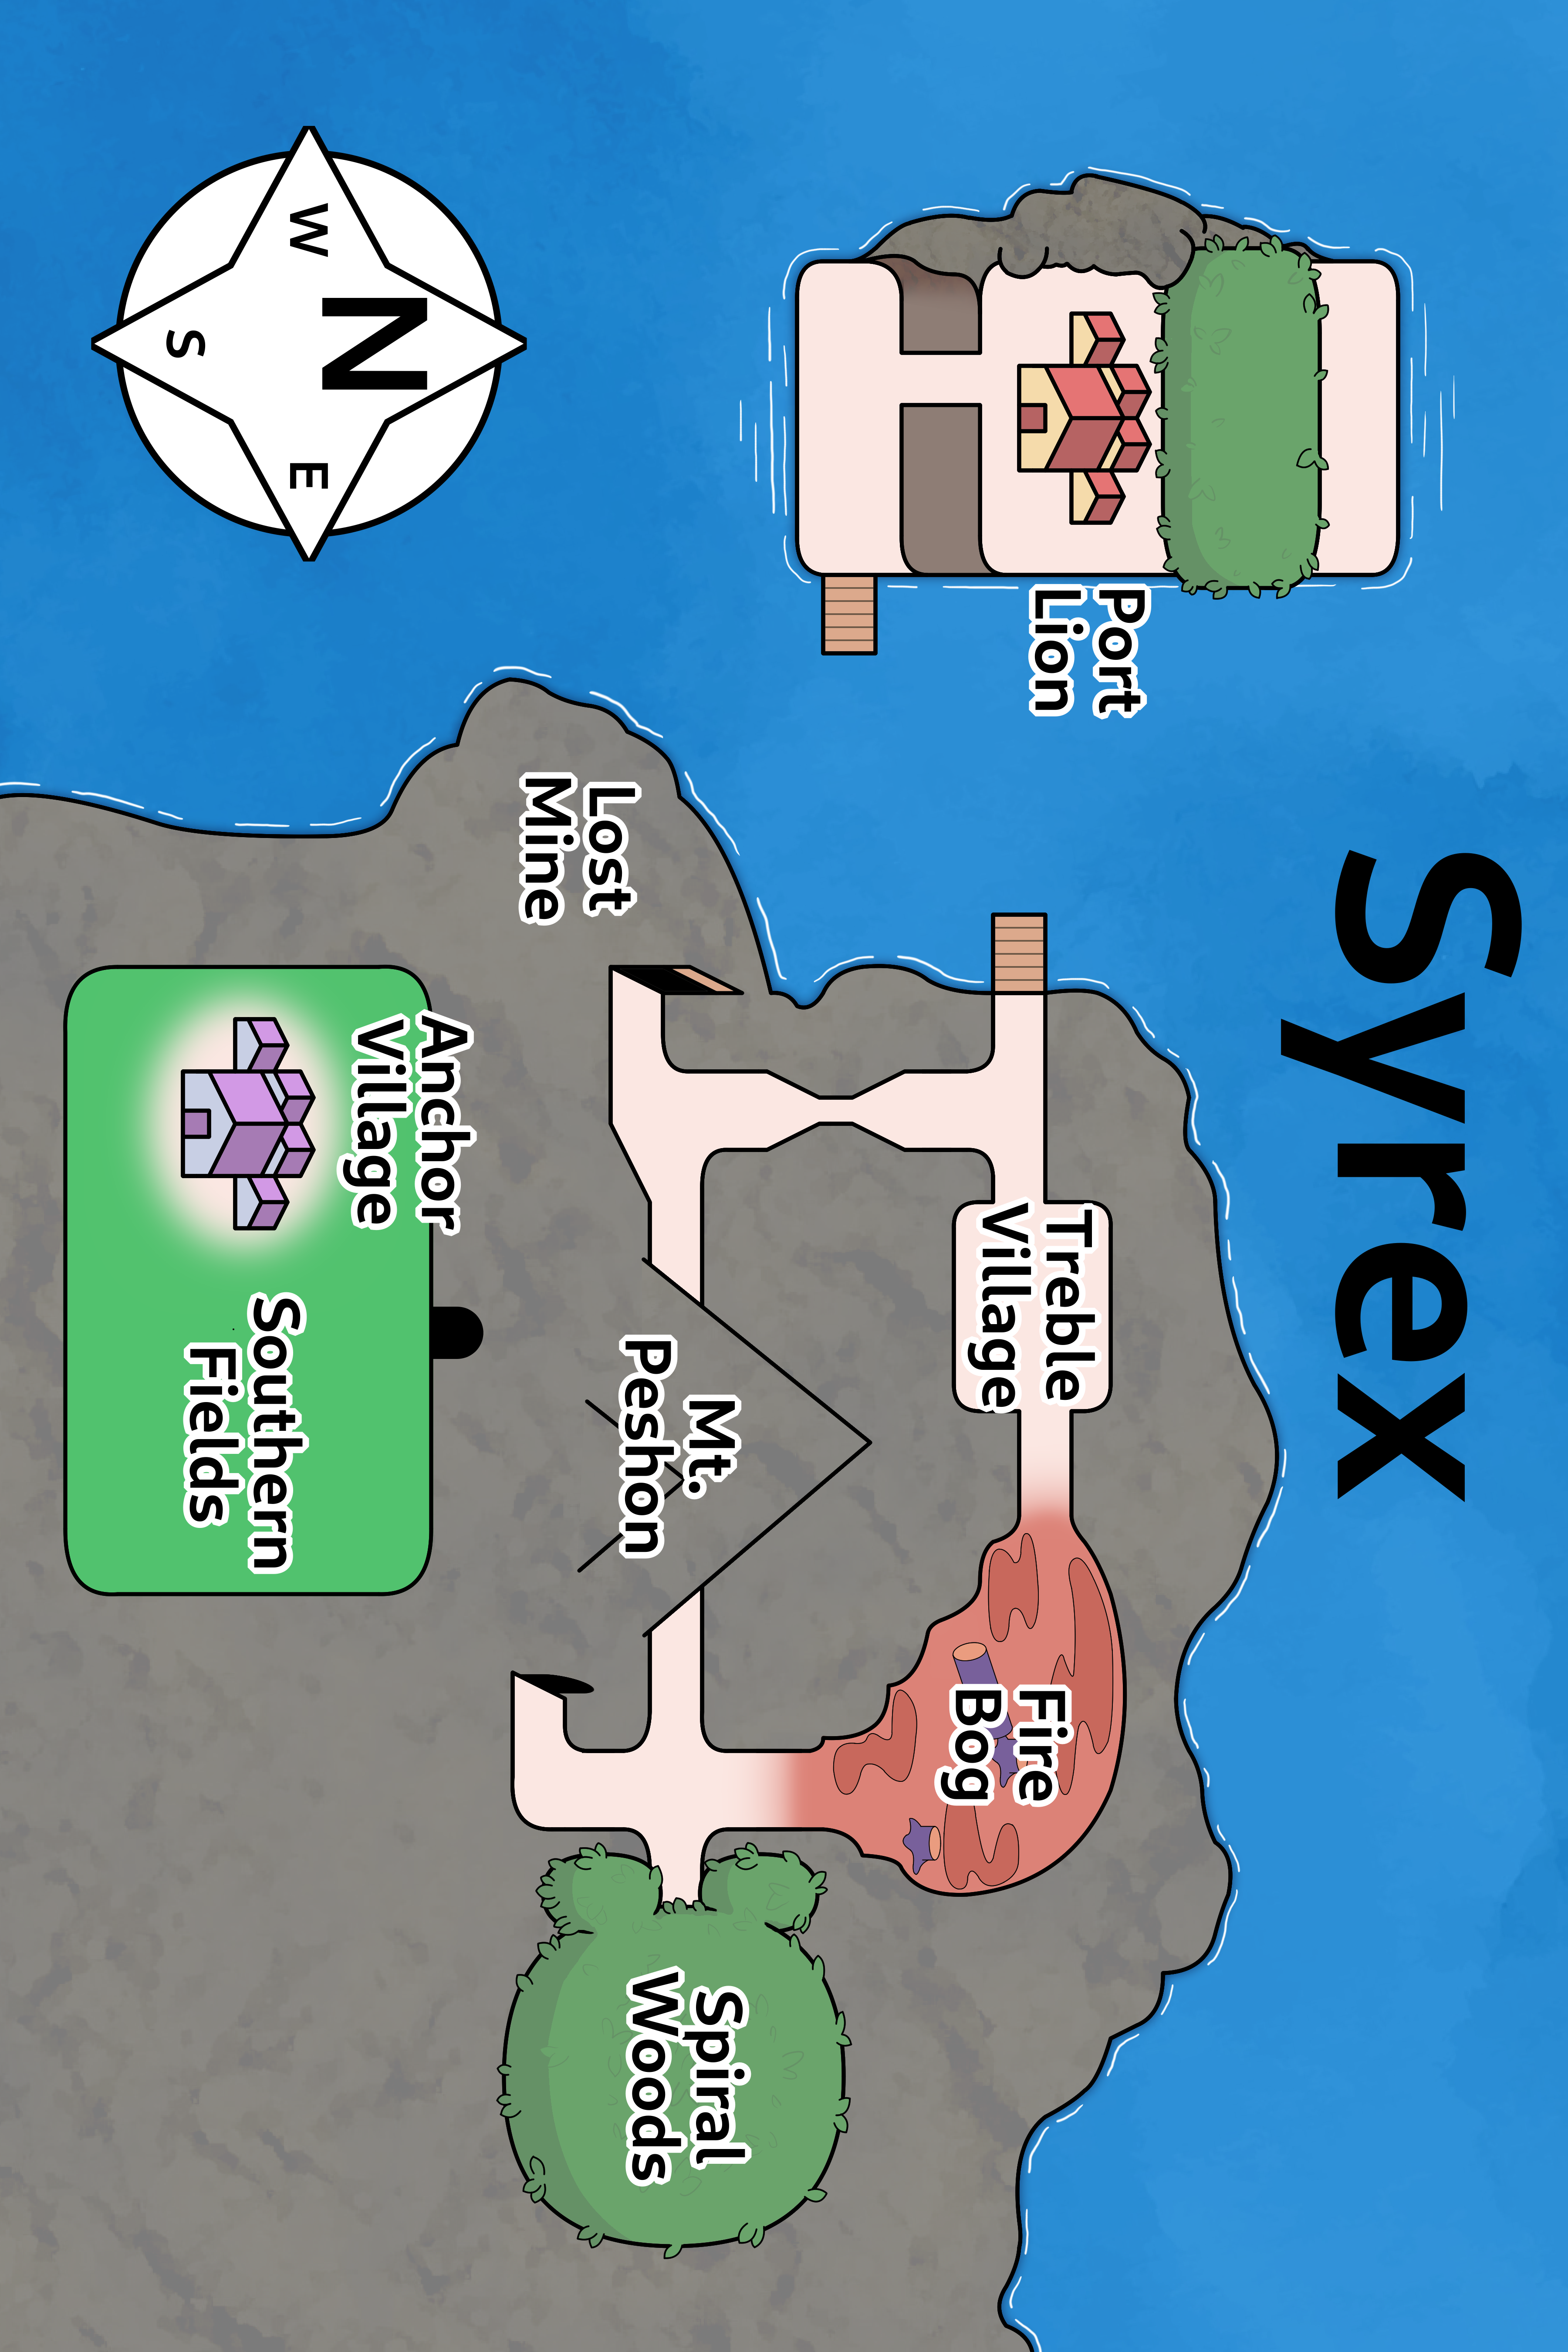
\includegraphics[interpolate,width=\paperwidth,height=\paperheight]{../Manual/SyrexMap.png}};
\end{tikzpicture}

\clearpage


\section{The Mainland}

This is where you begin the game, and takes up the eastern side of the map.

\subsection{Treble Village}

\begin{figure*}[ht]
  \begin{center}
    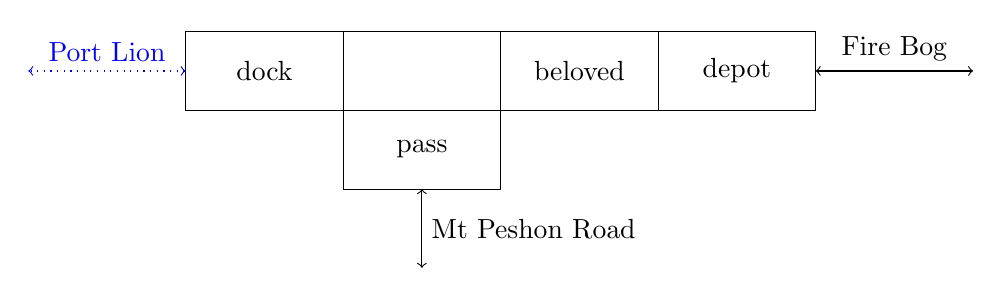
\begin{tikzpicture}
      \draw [<->, blue, dotted] (2, 1.5) -- (0, 1.5);
      \node [above, blue] at (1, 1.5) { Port Lion };
      \draw (2, 2) rectangle (6, 1);
      \node at (3, 1.5) { dock };
      \draw (4, 2) rectangle (6, 1);
      \draw (4, 0) rectangle (6, 1);
      \node at (5, .5) { pass };
      \draw (6, 2) rectangle (8, 1);
      \node at (7, 1.5) { beloved };
      \draw (8, 2) rectangle (10, 1);
      \node at (9, 1.5) { depot };
      \draw [<->] (10, 1.5) -- (12, 1.5);
      \node [above] at (11, 1.5) { Fire Bog };
      \draw [<->] (5, 0) -- (5, -1);
      \node [right] at (5, -.5) { Mt Peshon Road };
    \end{tikzpicture}
  \end{center}
  \addcontentsline{map}{map}{Map of Treble Village}
  \caption{Map of Treble Village}
\end{figure*}

Treble village has been destroyed almost completely by monsters, but a few brave
souls have hunkered  down. From the Grizzard  Depot in the east to  the docks in
the west, there isn't a single house left standing.

You'll   begin  the   game   in  the   ruins  of   Treble   village  with   your
Starting Grizzard.  You can only get  the two other Starter  Grizzards (the ones
you did not choose at first) by winning the game and beginning a New Game Plus.

\subsection{Fire Bog}

\begin{figure*}[ht]
  \begin{center}
    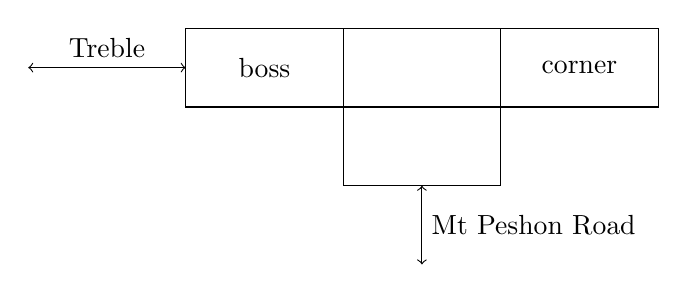
\begin{tikzpicture}
      \draw [<->] (2, 1.5) -- (0, 1.5);
      \node [above] at (1, 1.5) { Treble };
      \draw (2, 2) rectangle (4, 1);
      \node at (3, 1.5) { boss };
      \draw (4, 2) rectangle (6, 1);
      \draw (6, 2) rectangle (8, 1);
      \node at (7, 1.5) { corner };
      \draw (4, 1) rectangle (6, 0);
      \draw [<->] (5, 0) -- (5, -1);
      \node [right] at (5, -.5) { Mt Peshon Road };
    \end{tikzpicture}
  \end{center}
  \addcontentsline{map}{map}{Map of the Fire Bog}
  \caption{Map of the Fire Bog}
\end{figure*}

The dangerous Fire Bog is full of monsters. Watch your step, or Flame Doggos and
Rodents of Unusual Size may attack you.

Near  the west  side of  the Fire  Bog,  a Boss  Rodent of  Unusual Size  blocks
a  particularly winding  path. In  the east,  one of  the survivors  from Treble
Village has an artifact that you'll need to open the tunnels under Mount Peshon,
and you can also catch Flamex.

\subsection{Mount Peshon road}

\begin{figure*}[ht]
  \begin{center}
    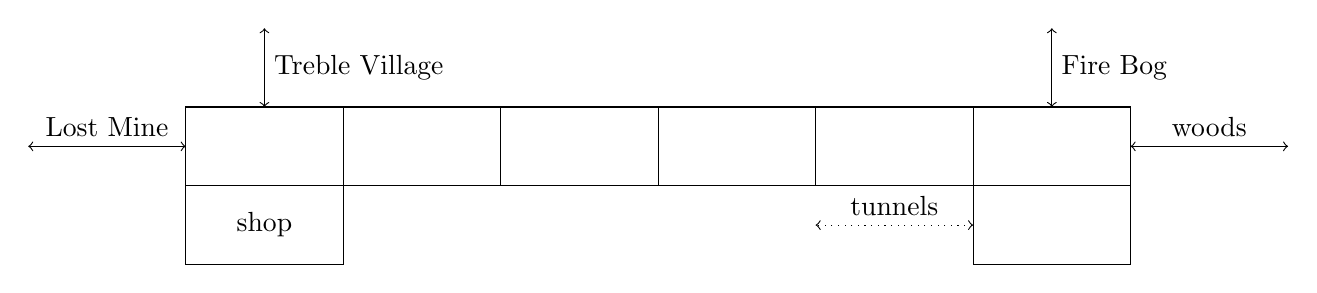
\begin{tikzpicture}
      \draw (10, 0) rectangle (12, 1);
      \draw [<->, dotted] (10, .5) -- (8, .5);
      \node [above] at (9, .5) { tunnels };
      \draw (10, 1) rectangle (12, 2);
      \draw [<->] (11, 2) -- (11, 3);
      \node [right] at (11, 2.5) { Fire Bog };
      \draw [<->] (12, 1.5) -- (14, 1.5);
      \node [above] at (13, 1.5) { woods };
      \draw (8, 1) rectangle (10, 2);
      \draw (6, 1) rectangle (8, 2);
      \draw (4, 1) rectangle (6, 2);
      \draw (2, 1) rectangle (4, 2);
      \draw (0, 1) rectangle (2, 2);
      \draw (0, 0) rectangle (2, 1);
      \node at (1, .5) { shop };
      \draw [<->] (0, 1.5) -- (-2, 1.5);
      \node [above] at (-1, 1.5) { Lost Mine };
      \draw [<->] (1, 2) -- (1, 3);
      \node [right] at (1, 2.5) { Treble Village };
    \end{tikzpicture}
  \end{center}
  \addcontentsline{map}{map}{Map of the Mount Peshon road}
  \caption{Map of the Mount Peshon road}
\end{figure*}

The road running along the north side of Mount Peshon reaches from the Lost Mine
in the west to the Spiral Woods in  the east. Near the Spiral Woods, a crossroad
joins up to the Fire Bog and the entrance to the Mount Peshon tunnels.

A lonely radio repair shop can be found near the Lost Mine entrance.

\subsection{Mount Peshon}

\begin{figure*}[ht]
  \begin{center}
    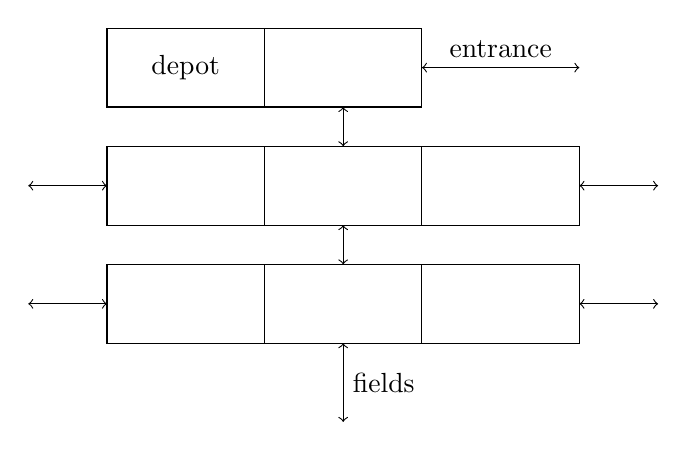
\begin{tikzpicture}
      \draw (4, 1) rectangle (6, 2);
      \draw [<->] (5, 1) -- (5, 0);
      \node [right] at (5, .5) { fields };
      \draw (2, 1) rectangle (4, 2);
      \draw [<->] (2, 1.5) -- (1, 1.5);
      \draw (6, 1) rectangle (8, 2);
      \draw [<->] (8, 1.5) -- (9, 1.5);

      \draw [<->] (5, 2) -- (5, 2.5);
      
      \draw (4, 2.5) rectangle (6, 3.5);
      \draw (2, 2.5) rectangle (4, 3.5);
      \draw [<->] (2, 3) -- (1, 3);
      \draw (6, 2.5) rectangle (8, 3.5);
      \draw [<->] (8, 3) -- (9, 3);

      \draw [<->] (5, 4) -- (5, 3.5);
      \draw (4, 4) rectangle (6, 5);
      \draw (2, 4) rectangle (4, 5);
      \node at (3, 4.5) { depot };
      \draw [<->] (6, 4.5) -- (8, 4.5);
      \node [above] at (7, 4.5) { entrance };
    \end{tikzpicture}
  \end{center}
  \addcontentsline{map}{map}{Map of the Mount Peshon tunnels}
  \caption{Map of the Mount Peshon tunnels}
\end{figure*}

Mount Peshon  divides the mainland into  a northern and southern  side. The only
way through are a series of tunnels beneath the mountain.

When the  game begins, the  tunnels cannot be  opened because the  two artifacts
used to open them, which were in Treble village, are missing.

If  you do  manage to  get into  the  tunnels, your  passage may  be blocked  by
emergency barricades  that are  put up whenever  a Grue is  heard in  the caves.
Nobody knows quite what a Grue looks  like, because they usually eat anyone that
comes across them, and they live in the dark places beneath Syrex.

It's  also been  known that  there are  side  caves off  the main  one in  which
a terrible Cyclops is raising a herd of venomous sheep.

\subsection{Spiral Woods}

\begin{figure*}[ht]
  \begin{center}
    \begin{tikzpicture}
      \draw (2, 4) rectangle (4, 5);
      \draw [<->] (1, 4.5) -- (2, 4.5);
      \node [above] at (1.5, 4.5) { crossroads };

      \draw (2, 3) rectangle (4, 4);
      \draw (2, 5) rectangle (4, 6);
      \node at (3, 5.5) { artifact };

      \draw [<->] (4, 4.5) -- (5, 4.5);

      \draw (5, 4) rectangle (7, 5);
      \draw [<->] (6, 5) -- (6, 6);
      \draw (5, 6) rectangle (7, 7);
      \draw [<->] (7, 6.5) -- (8, 6.5);
      \draw (8, 6) rectangle (10, 7);
      \draw [<->] (10, 6.5) -- (11, 6.5);
      \draw (11, 6) rectangle (13, 7);
      \draw [<->] (13, 6.5) -- (16.5, 6.5);
      \draw (16.5, 6) rectangle (18.5, 7);

      \draw [<->] (17.5, 6) -- (17.5, 5);
      \draw (16.5, 5) rectangle (18.5, 4);
      \draw [<->] (17.5, 4) -- (17.5, 3);
      \draw (16.5, 3) rectangle (18.5, 2);

      \draw [<->] (14,2.5) -- (16.5, 2.5);
      \draw (12, 2) rectangle (14, 3);
      \draw (10, 2) rectangle (12, 3);
      \draw (8, 2) rectangle (10, 3);

      \draw [<->] (8.5, 3) -- (8.5, 4);
      \draw (8, 4) rectangle (10, 5);
      \draw (10, 4) rectangle (12, 5);
      \draw (12, 4) rectangle (14, 5);
      \draw (14, 4) rectangle (16, 5);

      \node at (15, 4.5) { depot };
    \end{tikzpicture}
  \end{center}
  \addcontentsline{map}{map}{Map of the Spiral Woods}
  \caption{Map of the Spiral Woods}
\end{figure*}

The Spiral Woods are full of  Crazy Foxes, Vorpal Bunnies, and Will-O-Wisps, but
somewhere in the center of the forest is a Grizzard Depot.

One of  the survivors of Treble  Village can be  found in the Woods,  holding an
important artifact.

A Grizzard Trainer in Anchor village will  tell you that she's lost a pendant in
the Spiral Woods. If you find an  area with relatively few monsters, it might be
wise to search for that pendant --- there's sure to be a great reward.

Windoo can be found in the Spiral Woods.

\subsection{Southern Fields}

\begin{figure*}[ht]
  \begin{center}
    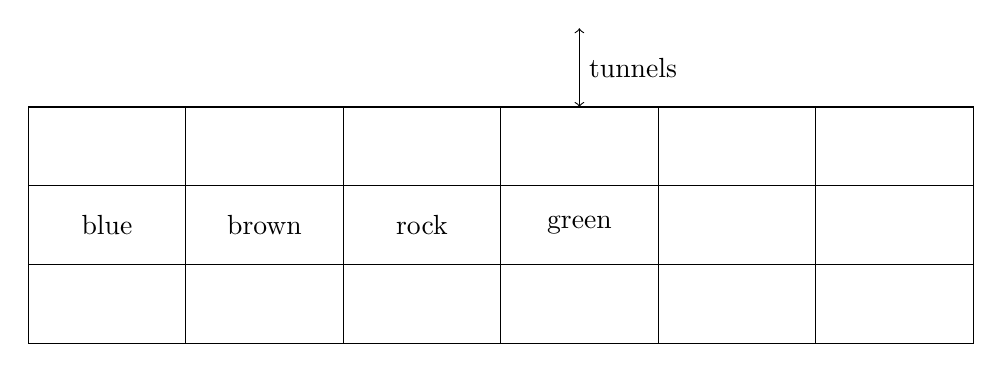
\begin{tikzpicture}
      \draw (0, 0) rectangle (2, 1);
      \draw (0, 1) rectangle (2, 2);
      \draw (0, 2) rectangle (2, 3);
      \draw (2, 0) rectangle (4, 1);
      \draw (2, 1) rectangle (4, 2);
      \draw (2, 2) rectangle (4, 3);
      \draw (4, 0) rectangle (6, 1);
      \draw (4, 1) rectangle (6, 2);
      \draw (4, 2) rectangle (6, 3);
      \draw (6, 0) rectangle (8, 1);
      \draw (6, 1) rectangle (8, 2);
      \draw (6, 2) rectangle (8, 3);
      \draw (8, 0) rectangle (10, 1);
      \draw (8, 1) rectangle (10, 2);
      \draw (8, 2) rectangle (10, 3);
      \draw (10, 0) rectangle (12, 1);
      \draw (10, 1) rectangle (12, 2);
      \draw (10, 2) rectangle (12, 3);

      \draw [<->] (7, 3) -- (7, 4);
      \node [right] at (7, 3.5) { tunnels };

      \node at (1, 1.5) { blue };
      \node at (3, 1.5) { brown };
      \node at (5, 1.5) { rock };
      \node at (7, 1.5) { green };
    \end{tikzpicture}
  \end{center}
  \addcontentsline{map}{map}{Map of the Southern Field and Anchor Village}
  \caption{Map of the Southern Field and Anchor Village}
\end{figure*}

The Southern Fields are beset with monsters, too, now, but they haven't yet come
up into Anchor Village.

The  only  way  in  or  out  of   the  Southern  Fields  is  through  the  Mount
Peshon tunnel, but there is a hidden cave into Mount Peshon as well. If you find
the key to revealing the cave's entrance, you'll also discover a hidden Grizzard
Depot nearby.

\subsection{Anchor Village}

Still mostly  unharmed by the  monsters, Anchor  Village is built  around Anchor
Rock, a large red monolith from the ancient past.

Villagers here can be very helpful,  manufacturing potions, using their radio to
call ships  to the Treble  village docks, or even  giving you access  to trained
Grizzards that they no longer need: Cornet, Ambren, and Noctis.

\section{Lost Mine}

Delving deep into the underworld, the Lost Mine is a maze in which it is far too
easy to lose yourself. Even going back the  way in which you came might take you
someplace different, if you're not careful.

Somewhere in the mine can be found Splodo, near an abandoned Grizzard Depot.

Mapping  the Lost  Mine does  \emph{not} work  on a  graph paper,  and wandering
through it's unlikely  that you'll find what you're looking-for  --- but someone
must know the secret to navigating its passages. Perhaps someone in Anchor village?

\section{Port Lion}

The island of  Port Lion is home to  the village of Port Lion,  and is reachable
via a ship from the Treble docks.

\begin{figure*}[ht]
  \begin{center}
    \begin{tikzpicture}
      \draw (0,0) rectangle (10,10);
    \end{tikzpicture}
  \end{center}
  \addcontentsline{map}{map}{Map of Port Lion}
  \caption{Map of Port Lion}
\end{figure*}

\subsection{South Beaches}

One  the south  beaches  of  Port Lion  are  quite a  few  monsters  --- and  an
opportunity, on the docks,  to meet Fat Tony, who (as he  will tell you himself)
is the local expert on the geography of Port Lion.

Firend can be caught on the west end of the beach.

\subsection{Cliffs}

The village  of Port  Lion is  found atop some  high cliffs  that loom  over the
south beaches. There are a couple of paths up to the cliff-tops.

Fat  Tony will  tell  you about  a  legend  about one  area  of the  cliff-tops.
Perhaps it might be significant?

\subsection{Port Lion Village}

The village  of Port Lion is  a bustling community  that so far has  escaped the
notice of the monsters --- but for how long?

The villagers are fairly gossipy. Perhaps  if you solve the latest town mystery,
they can give you more information?

One villager's home has a Grizzard Depot inside, and he will cheerfully offer to
teach any Grizzard its last move. Since that is always its most powerful healing
move, that can be quite helpful.

\subsection{Lion Woods}

The Lion  Woods on  the north of  Port Lion  are a small  forest with  many evil
monsters prowling through it.

Corlyn can be found in the woods, if you search long enough.

\subsection{North Beaches}

Despite the plague of  monsters, some Port Lion residents still  try to fish off
the north  beaches. I wonder  what things other  than fish (and  monsters) might
turn up?

\section{Labyrinth}

\begin{figure*}[ht]
  \begin{center}
    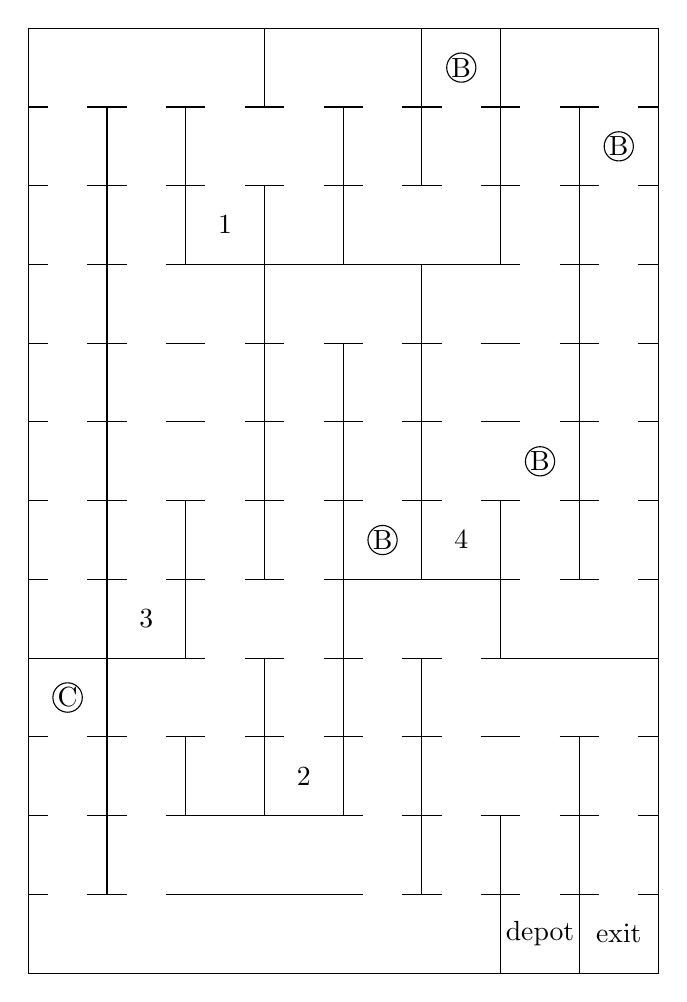
\begin{tikzpicture}
      \foreach \x in {0,...,7}
      { \foreach \y in {0,...,11}
        { \draw (\x,\y) -- (\x+.25,\y);
          \draw (\x+.75,\y) -- (\x+1,\y); } }
      \draw (0,0) rectangle (8,12);
      \draw (1,1) -- (1,4);
      \draw (0,4) -- (2,4);
      \draw (2,4) -- (2,6);
      \draw (1,3) -- (1,11);
      \draw (2,1) -- (4,1);
      \draw (6,0) -- (6,2);
      \draw (7,0) -- (7,3);
      \draw (5,1) -- (5,4);
      \draw (2,2) -- (2,3);
      \draw (2,2) -- (4,2) -- (4,8);
      \draw (3,2) -- (3,4);
      \draw (4,5) -- (6,5) -- (6,4) -- (8,4);
      \draw (5,5) -- (5,9);
      \draw (5,10) -- (5,12);
      \draw (2,11) -- (2,9) -- (6,9) -- (6,12);
      \draw (3,11) -- (3,12);
      \draw (3,5) -- (3,10);
      \draw (4,9) -- (4,11);
      \draw (7,5) -- (7,11);
      \draw (6,5) -- (6,6);
      \node at (.5,3.5) { \encircle{C} };
      \node at (7.5,.5) { exit };
      \node at (2.5,9.5) { 1 };
      \node at (3.5,2.5) { 2 };
      \node at (1.5,4.5) { 3 };
      \node at (5.5,5.5) { 4 };
      \node at (6.5,.5) { depot };
      \node at (4.5,5.5) { \encircle{B} };
      \node at (6.5,6.5) { \encircle{B} };
      \node at (7.5,10.5) { \encircle{B} };
      \node at (5.5,11.5) { \encircle{B} };
    \end{tikzpicture}
  \end{center}
  \addcontentsline{map}{map}{Map of Labyrinth Upper Level ``A''}
  \caption{Labyrinth Upper Level ``A'' (Blue)}
\end{figure*}

\begin{figure*}[ht]
  \begin{center}
    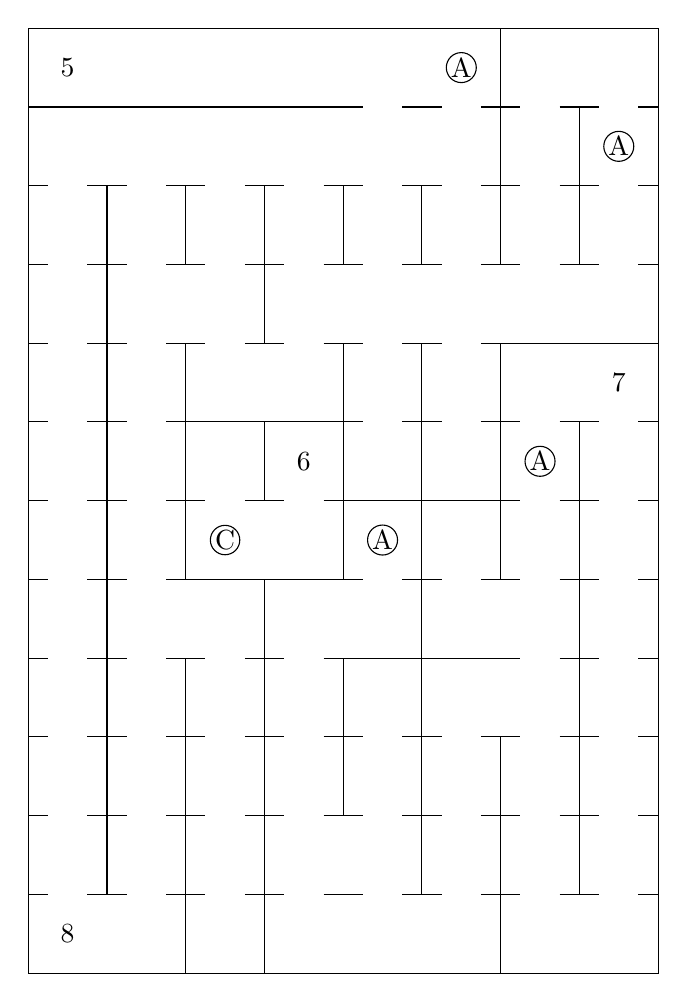
\begin{tikzpicture}
      \foreach \x in {0,...,7}
      { \foreach \y in {1,...,11}
        { \draw (\x,\y) -- (\x+.25,\y);
          \draw (\x+.75,\y) -- (\x+1,\y); } }
      \draw (0,0) rectangle (8,12);
      \draw (1,1) -- (1,10);
      \draw (0,11) -- (4, 11);
      \draw (2,0) -- (2,4);
      \draw (3,0) -- (3,5);
      \draw (2,9) -- (2,10);
      \draw (2,8) -- (2,5) -- (4,5) -- (4,8);
      \draw (2,7) -- (4,7);
      \draw (3,6) -- (3,7);
      \draw (3,8) -- (3,10);
      \draw (4,9) -- (4,10);
      \draw (5,9) -- (5,10);
      \draw (6,9) -- (6,12);
      \draw (7,9) -- (7,11);
      \draw (4,6) -- (6,6);
      \draw (5,1) -- (5,8);
      \draw (6,0) -- (6,3);
      \draw (4,2) -- (4,4) -- (6,4);
      \draw (7,1) -- (7,7);
      \draw (6,5) -- (6,8) -- (8,8);
      \node at (2.5,5.5) { \encircle{C} };
      \node at (4.5,5.5) { \encircle{A} };
      \node at (6.5,6.5) { \encircle{A} };
      \node at (5.5,11.5) { \encircle{A} };
      \node at (7.5,10.5) { \encircle{A} };
      \node at (.5,11.5) { 5 };
      \node at (3.5,6.5) { 6 };
      \node at (7.5,7.5) { 7 };
      \node at (.5,.5) { 8 };
    \end{tikzpicture}
  \end{center}
  \addcontentsline{map}{map}{Map of Labyrinth Mid Level ``B''}
  \caption{Labyrinth Mid Level ``B'' (Indigo)}
\end{figure*}

\begin{figure*}[ht]
  \begin{center}
    \begin{tikzpicture}
      \foreach \x in {2,...,3}
      { \foreach \y in {4,...,5}
        { \draw (\x,\y) -- (\x+.25,\y);
          \draw (\x+.75,\y) -- (\x+1,\y); } }
      \foreach \x in {0,...,5}
      { \foreach \y in {1,...,3}
        { \draw (\x,\y) -- (\x+.25,\y);
          \draw (\x+.75,\y) -- (\x+1,\y); } }
      \draw (4,4) -- (6,4) -- (6,0) -- (0,0) -- (0,4) -- (2,4);
      \draw (2,3) -- (2,6) -- (4,6) -- (4,1);
      \draw (1,4) -- (1,1);
      \draw (5,0) -- (5,1);
      \draw (2,0) -- (2,2);
      \draw (3,1) -- (3,2);
      \draw (3,4) -- (3,5);
      \draw (5,2) -- (5,4);
      \node at (.5,3.5) { \encircle{A} };
      \node at (2.5,5.5) { \encircle{B} };
      \node at (4.5,3.5) { 9 };
      \node at (5.5,.5) { 10 };
    \end{tikzpicture}
  \end{center}
  \addcontentsline{map}{map}{Map of Labyrinth Lower Level ``C''}
  \caption{Labyrinth Lower Level ``C'' (Purple)}
\end{figure*}

Ancient legends tell of a mysterious labyrinth in WRITEME


\subsection{References on Labyrinth maps}

\begin{description}
\item[exit]
  Stairs up to the surface
\item[depot]
  A Grizzard Depot
\item[\encircle{A}]
  Stairs to Upper Level ``A'' (Blue)
\item[\encircle{B}]
  Stairs to Mid Level ``B'' (Indigo)
\item[\encircle{C}]
  Stairs to Lower Level ``C'' (Purple)
\item[1]
  Sign that tells you where to find Andrew's lair
\item[2]
  Sign that tells you where to find Timmy's lair
\item[3]
  Lever to open Timmy's lair
\item[4]
  Guide to reading runes
\item[5]
  Entrance to Andrew's lair
\item[6]
  Entrance to Timmy's lair
\item[7]
  Lever to open Andrew's lair
\item[8]
  Entrance to Fred's lair
\item[9]
  Lever to open Fred's lair
\item[10]
  Sign that tells you where to find Fred's lair
\end{description}

\section{Dragons' Lairs}

The   lairs  of   the  three   dragons  are   accessible  only   through
the Labyrinth. Each  dragon's lair has a Grizzard Depot  and an arena in
which you can fight the dragon.

These lairs  are actually located  high above  the cliffs of  Port Lion.
You might notice  that the Port Lion  music can be heard  when you're in
these  lairs,   rather  than  the   underworld  music  that   you  might
have expected.

\chapter{Moves}\label{ch:Moves}

There are 64 Moves which can be used by Grizzards and monsters alike.

\section{Run Away}

You can run away from a fight, as long as the opposing monster is not a
Boss monster.

Running away does not heal your  Grizzard, but it does remove any Status
Effects that they may have received  (eg. Attack Down) during the fight.
It \emph{does},  however, allow the  monsters to fully  heal themselves,
and even  gather their forces ---  if you had  killed one of a  group of
monsters, a new one of the same kind will come to take its place.

\section{Grizzards' Moves}\label{sec:GrizzardMoves}

Each Grizzard is capable of learning  up to eight moves. There are three
ways to learn a move:

\begin{itemize}
\item Your Grizzard will know certain Moves when you first catch them.
\item When  a monster  uses a  Move against you  (or on  themself), your
  Grizzard can observe them and learn the Move from the monster.
\item Sometimes,  when gaining experience  by defeating a  monster, your
  Grizzard  will  spontaneously  discover  how  to  perform  a  Move  on
  their  own.  This occurs  less  frequently  than  learning a  Move  by
  observation, but it can happen.
\end{itemize}

The following shows all of the Moves that each Grizzard can learn.
See the  moves dictionary  starting on  page~\pageref{sec:MovesTable} to
see what the effects of each move can be.

\begin{description}

\newcommand\grizzardmoves[9]{%
\item[#1]
#2, #3, #4, #5, #6, #7, #8, #9, and Run Away
}
\grizzardmoves{Airex}{Mild Shock}{Wind Fight}{Steal Attack}{Steal Defend}{Steal Turn}{Burnt Edges}{First Aid}{Simple Cure}
\grizzardmoves{Altrix}{Crush}{Sharp Fangs}{Talon Vise}{Hard Tackle}{Head Butt}{Great Cure}{Heal Wound}{Life Return}
\grizzardmoves{Ambren}{Claws Out}{Bite}{Hearty Thump}{Hard Jab}{Stomp Down}{Common Cure}{Great Cure}{Heal Wound}
\grizzardmoves{Aquax}{Splish Splash}{Raise Hope}{Sure Splash}{Quick Foot}{Great Mojo}{First Aid}{Simple Cure}{Common Cure}
\grizzardmoves{Burner}{Hot Spark}{Fire Start}{Burnt Edges}{Rogue Flare}{Double Flares}{Simple Cure}{Common Cure}{Great Cure}
\grizzardmoves{Corlyn}{Burnt Edges}{Shove}{Bite}{Slash}{Stomp Down}{Common Cure}{Great Cure}{Heal Wound}
\grizzardmoves{Cornet}{Tail Lash}{Bite}{Hearty Thump}{Slash}{Claw Badly}{Common Cure}{Great Cure}{Heal Wound}
\grizzardmoves{Dirtex}{Kick Dirt}{Bury Deep}{Dirty Foot}{Loamy Fear}{Dusty Eyes}{Shove}{First Aid}{Simple Cure}
\grizzardmoves{Dufont}{Poison Bite}{Head Butt}{Crush}{Evil Eye}{Sharp Fangs}{Great Cure}{Heal Wound}{Life Return}
\grizzardmoves{Ectrix}{Cruel Stab}{Talon Vise}{Crush}{Sharp Fangs}{Head Butt}{Great Cure}{Heal Wound}{Life Return}
\grizzardmoves{Firend}{Hot Spark}{Fire Start}{Burnt Edges}{Rogue Flare}{Double Flares}{Simple Cure}{Common Cure}{Great Cure}
\grizzardmoves{Flamex}{Hot Spark}{Fire Start}{Burnt Edges}{Rogue Flare}{Double Flares}{Simple Cure}{Common Cure}{Great Cure}
\grizzardmoves{Flarex}{Rogue Flare}{Double Flares}{Slash}{Hard Jab}{Claw Badly}{Great Cure}{Heal Wound}{Life Return}
\grizzardmoves{Flitex}{Hard Jab}{Slash}{Hearty Thump}{Stomp Down}{Claw Badly}{Great Cure}{Heal Wound}{Life Return}
\grizzardmoves{Flyer}{Steal Defend}{Steal Turn}{Tail Whip}{Tail Lash}{Rogue Flare}{Simple Cure}{Common Cure}{Great Cure}
\grizzardmoves{Lander}{Dirty Foot}{Loamy Fear}{Dusty Eyes}{Shove}{Pound Sand}{Simple Cure}{Common Cure}{Great Cure}
\grizzardmoves{Megax}{Bite}{Stomp Down}{Crush}{Evil Eye}{Mega Kill}{Great Cure}{Heal Wound}{Life Return}
\grizzardmoves{Noctis}{Bite}{Hearty Thump}{Slash}{Hard Jab}{Claw Badly}{Common Cure}{Great Cure}{Heal Wound}
\grizzardmoves{Oceax}{Slash}{Claw Badly}{Cruel Stab}{Poison Bite}{Crush}{Great Cure}{Heal Wound}{Life Return}
\grizzardmoves{Ortrix}{Head Butt}{Poison Bite}{Evil Eye}{Hard Tackle}{Crush}{Great Cure}{Heal Wound}{Life Return}
\grizzardmoves{Sailor}{Sure Splash}{Quick Foot}{Great Mojo}{Wet Noodle}{First Aid}{Simple Cure}{Common Cure}{Great Cure}
\grizzardmoves{Soiley}{Dirty Foot}{Loamy Fear}{Dusty Eyes}{Tail Whip}{First Aid}{Simple Cure}{Common Cure}{Great Cure}
\grizzardmoves{Splodo}{Bite}{Rogue Flare}{Double Flares}{Firey Breath}{Fire Start}{Tail Whip}{Nibble}{Life Return}
\grizzardmoves{Theref}{Hard Tackle}{Poison Bite}{Head Butt}{Crush}{Evil Eye}{Stomp Down}{Cruel Stab}{Life Return}
\grizzardmoves{Tyrant}{Head Butt}{Crush}{Sharp Fangs}{Death Glare}{Back Kick}{Great Cure}{Heal Wound}{Life Return}
\grizzardmoves{Uptrix}{Head Butt}{Hard Tackle}{Sharp Fangs}{Talon Vise}{Cruel Stab}{Great Cure}{Heal Wound}{Life Return}
\grizzardmoves{Wapow}{Sharp Fangs}{Crush}{Head Butt}{Back Kick}{Stomp Down}{Great Cure}{Heal Wound}{Life Return}
\grizzardmoves{Wetnas}{Great Mojo}{Quick Foot}{Sure Splash}{Wet Noodle}{First Aid}{Simple Cure}{Common Cure}{Great Cure}
\grizzardmoves{Windoo}{Tail Whip}{Tail Lash}{Steal Defend}{Steal Turn}{First Aid}{Simple Cure}{Common Cure}{Great Cure}
\grizzardmoves{Zendex}{Stomp Down}{Claw Badly}{Cruel Stab}{Back Kick}{Head Butt}{Great Cure}{Heal Wound}{Life Return}

\end{description}

\section{Monsters' Moves}\label{sec:MonsterMoves}

Monsters each  know only four Moves.  They will use attack  moves first,
and resort to healing Moves (if they know any) only when injured.

Boss monsters know the same Moves as their lesser, non-boss variety, but
of course they have higher stats.

The following table shows all of the Moves that each monster can use.

Boss monsters have the same moves as the common monsters of the same
type.

Some monsters know less than four distinct moves. For examples, a Wicked
Slime is twice as likely to pick Splish Splash as it occupies two of its
move slots.

\begin{description}
\newcommand\monstermoves[5]{%
\item[#1]
  #2, #3, #4, and #5
}

\monstermoves{Anubis Jackal}{Firey Breath}{Nasty Goop}{Death Glare}{Great Cure}
\monstermoves{Bigger Crab}{Crush}{Head Butt}{Pirate Curse}{Common Cure}
\monstermoves{Boss Bear}{Firey Breath}{Evil Eye}{Sharp Fangs}{Death Glare}
\monstermoves{Butterfly}{Double Flares}{Slash}{Wings Flap}{Common Cure}
\monstermoves{Cave Bat}{Deadly Swoop}{Nibble}{Great Mojo}{Burnt Edges}
\monstermoves{Cave Grue}{Tail Whip}{Nibble}{Great Mojo}{Shove}
\monstermoves{Crazy Fox}{Tail Lash}{Claws Out}{Rogue Flare}{Nibble}
\monstermoves{Crazy Skull}{Firey Breath}{Death Glare}{Pirate Curse}{Death Glare}
\monstermoves{Creepy Spider}{Bite}{Vampy Bite}{Nibble}{Common Cure}
\monstermoves{Devil Skull}{Poison Bite}{Head Butt}{Cursed Glance}{Common Cure}
\monstermoves{Dragon Andrew}{Stomp Down}{Crush}{Firey Breath}{Evil Eye}
\monstermoves{Dragon Fred}{Stomp Down}{Crush}{Firey Breath}{Evil Eye}
\monstermoves{Dragon Timmy}{Stomp Down}{Crush}{Firey Breath}{Evil Eye}
\monstermoves{Fierce Raptor}{Claw Badly}{Slash}{Bite}{Simple Cure}
\monstermoves{Fire Drake}{Back Kick}{Double Flares}{Claw Badly}{Common Cure}
\monstermoves{Fire Panda}{Hot Spark}{Quick Foot}{Wind Fight}{Simple Cure}
\monstermoves{Flame Doggo}{Hot Spark}{Dirty Foot}{Quick Foot}{Simple Cure}
\monstermoves{Flying Skull}{Pirate Curse}{Pirate Curse}{Head Butt}{Poison Bite}
\monstermoves{Giant  Slime}{Slime   Impact}{Slime  Impact}{Slime  Impact}{Common  Cure}
\monstermoves{Giant Bat}{Evil Eye}{Talon Vise}{Talon Vise}{Great Cure}
\monstermoves{Giant Crab}{Slash}{Hard Jab}{Hearty Thump}{Bite}
\monstermoves{Giant Spider}{Death Glare}{Sharp Fangs}{Death Glare}{Great Cure}
\monstermoves{Grabby Crabby}{Slash}{Hard Jab}{Claws Out}{Pound Sand}
\monstermoves{Great Wyrm}{Evil Eye}{Sharp Fangs}{Evil Eye}{Great Cure}
\monstermoves{Horrid Slime}{Splish Splash}{Slimy Trick}{Blind Blob}{First Aid}
\monstermoves{Lectro Sheep}{Back Kick}{Cursed Glance}{Hearty Thump}{Common Cure}
\monstermoves{Leggy Mutant}{Cruel Stab}{Back Kick}{Stomp Down}{Simple Cure}
\monstermoves{Man Bull}{Head Butt}{Cruel Stab}{Stomp Down}{Head Butt}
\monstermoves{Maze Jaguar}{Evil Eye}{Sharp Fangs}{Crush}{Great Cure}
\monstermoves{Mean Robber}{Hearty Thump}{Pound Sand}{Common Cure}{Great Muddle}
\monstermoves{Metal Mouse}{Bite}{Claws Out}{Tail Lash}{Simple Cure}
\monstermoves{One-Eyed Cyclops}{Pound Sand}{Wet Noodle}{Rogue Flare}{Great Muddle}
\monstermoves{Poison Asp}{Poison Bite}{Poison Bite}{Poison Bite}{Great Cure}
\monstermoves{Radish Goblin}{Tail Lash}{Pound Sand}{Nibble}{Simple Cure}
\monstermoves{Rodent of Unusual Size}{Dirty Foot}{Quick Foot}{Common Cure}{Kick Dirt}
\monstermoves{Round Robin}{First Aid}{Mild Shock}{Splish Splash}{Kick Dirt}
\monstermoves{Scary Rat}{Poison Bite}{Cursed Glance}{Claw Badly}{Slash}
\monstermoves{Sky Mutant}{Hot Spark}{Mild Shock}{Splish Splash}{Kick Dirt}
\monstermoves{Turnip Goblin}{Poison Bite}{Cursed Glance}{Stomp Down}{Great Cure}
\monstermoves{Uber Slime}{Slime Impact}{Slime Impact}{Nasty Goop}{Nasty Goop}
\monstermoves{Venom Sheep}{Wet Noodle}{Rogue Flare}{First Aid}{Common Cure}
\monstermoves{Viking Turtle}{Claws Out}{Tail Lash}{Pound Sand}{Common Cure}
\monstermoves{Vorpal Bunny}{Great Mojo}{Shove}{Quick Foot}{Simple Cure}
\monstermoves{Water Kitty}{Slash}{Bite}{Claws Out}{Common Cure}
\monstermoves{Wicked Slime}{Splish Splash}{Splish Splash}{Slimy Trick}{First Aid}
\monstermoves{Will-O-Wisp}{Burnt Edges}{Great Muddle}{Hot Spark}{Simple Cure}

\end{description}

\section{Moves' Effects}\label{sec:MovesTable}

Each  Move can  cause  damage,  or healing,  and  can  also impart  some
temporary  Status   Effects.  This  table  enumerates   every  Move  and
their effects.

The actual  amount of damage or  healing will vary somewhat;  the values
shown are the base amounts. Healing moves will always heal at least 1 HP.

\subsection{Effectiveness}

Moves have a base effectiveness, shown in the following tables. However,
their base  effectiveness is modified by  a random factor. This  is like
``rolling  for  damage''   in  a  tabletop  RPG.  The   exact  range  of
effectiveness  of  any  Move  can  be determined  based  upon  its  base
effectiveness with the following table:

\begin{tabular}{l c}
  Base Effectiveness & Random Modifier \\
  1 - 3 & $\pm 1$ \\
  4 - 7 & $\pm 3$ \\
  8 - 15 & $\pm 7$ \\
  16 - 31 & $\pm 15$ \\
  32 - 63 & $\pm 31$ \\
  64 + & $\pm 63$ \\
\end{tabular}

\subsection{Defensive Moves}

These Moves are used by a creature on themself.

\begin{tabular}{l c l}
  Move & Healing & Status Effects \\
  Common Cure & 10 & \\
  Fire Start & & Attack Up \\
  First Aid & 2 & \\
  Great Cure & 25 & \\
  Heal Wound & 50 & \\
  Life Return & 99 & \\
  Raise Hope & & Defend Up \\
  Run Away & & (run away) \\
  Simple Cure & 5 & \\
  Sure Splash & & Attack Up \\
\end{tabular}

\subsection{Attack Moves}

These Moves are used against an enemy creature.

\begin{tabular}{l c l}
             Move & Damage & Status Effects \\
             Back Kick & 22 & \\
             Bite & 16 & \\
             Blind Blob & & Attack Down, Defend Down \\
             Burnt Edges & 8 & \\
             Bury Deep & 1 & Sleep \\
             Claw Badly & 20 & \\
             Claws Out & 14 & Defend Down \\
             Cruel Stab & 22 & \\
             Crush & 26 & \\
             Cursed Glance & 22 & Sleep \\
             Deadly Swoop & 10 & \\
             Death Glare & 30 & \\
             Dirty Foot & 6 & Defend Down \\
             Double Flares & 18 & \\
             Dusty Eyes & & Defend Down \\
             Evil Eye & 28 & Muddle \\
             Firey Breath & 30 & \\
             Great Mojo & 8 & Attack Down \\
             Great Muddle & 8 & \\
             Guard Down & & Defend Down \\
             Hard Jab & 16 & \\
             Hard Tackle & 29 & \\
             Head Butt & 24 & \\
             Hearty Thump & 16 & \\
             Hot Spark & 4 & \\
             Kick Dirt & 2 & \\
             Loamy Fear & & Attack Down \\
             Mega Kill & 50 & Defend Down, Attack Down, \\ & & Muddle, Sleep \\
             Mild Shock & 2 & \\
             Muddle Mind & & Muddle \\
             Nasty Goop & 30 & \\
             Nibble & 10 & \\
             Pirate Curse & 26 & Muddle, Sleep \\
             Poison Bite & 24 & Sleep \\
             Pound Sand & 12 & \\
             Quick Foot & 6 & Defend Down \\
             Rogue Flare & 12 & \\
             Sharp Fangs & 28 & \\
             Shove & 8 & \\
             Slash & 18 & \\
             Slime Impact & 26 & Muddle \\
             Slimy Trick & & Attack Down \\
             Splish Splash & 2 & \\
             Steal Attack & & Attack Down \\
             Steal Defend & & Defend Down \\
             Steal Turn & & Sleep \\
             Stomp Down & 20 & Sleep, Defend Down\\
             Tail Lash & 14 & \\
             Tail Whip & 10 & \\
             Talon Vise & 28 & \\
             Vampy Bite & 14 & Sleep \\
             Wet Noodle & 12 & \\
             Wind Fight & 6 & \\
             Wings Flap & 16 & \\
\end{tabular}

\end{document}
